\documentclass[a4paper,12pt,twocolumn]{report}
\usepackage[utf8]{inputenc}
\usepackage{graphicx}
\usepackage{natbib}   % omit 'round' option if you prefer square brackets
\usepackage{hyperref}
\graphicspath{ {img/} }


% Title Page
\title{CM30229 - Circumnavigation using Lejos}
\author{Dominic Hauton}


\begin{document}
\maketitle
\bibliographystyle{plainnat}

\section{Introduction}
% All of your courseworks are designed primarily to give you experience in developing intelligent control and/or cognitive systems. However, the course is also intended to give you experience and feedback in writing about research. To this end, you will be writing research reports of about two pages, using exactly this format.

% The Introduction of a research report should give a brief description of what you you tried to do (your hypothesis), and the outcome. It should also give some idea about why you have done it (motivation). In doing this, you may also give a brief background argument. I expect you to cite a paper or two for this motivational context. For coursework 1, one of the papers you should probably cite is Brooks (1991), since you have been asked to take a fairly reactive approach to developing robot intelligence.

% Coursework one requires you to construct a robot capable of circumnavigating rooms or other closed spaces (don’t worry about doorways – just close or block them.) Ideally this should work in “natural” (unaltered) indoor environments with a variety of obstacles along the walls, but often people build up some barriers. However, the report should not be about the entire experience of building a robot, but rather it should present a single hypothesis you tested on your completed robot about how to improve its intelligence.

The goal of this research is to see the effect of changing the rate of sensing on the navigation capabilities of the rover while circumnavigating a room. The rover was built using parts from the LEGO Mindstorm NXJ kit. There were 3 sensors; a \emph{Sonar}, \emph{Light Sensor} and \emph{Bump Sensor} (x3). Three motors were provided for movement and navigation.

To make informed decisions all of the sensors were used and the sonar was mounted on a pivot to allow for measurements in multiple directions, as shown in figure \ref{fig:stanley-head}. To provide movement two driven wheels were used and a trolley wheel was placed at the back for stability.

\begin{figure}[b]
 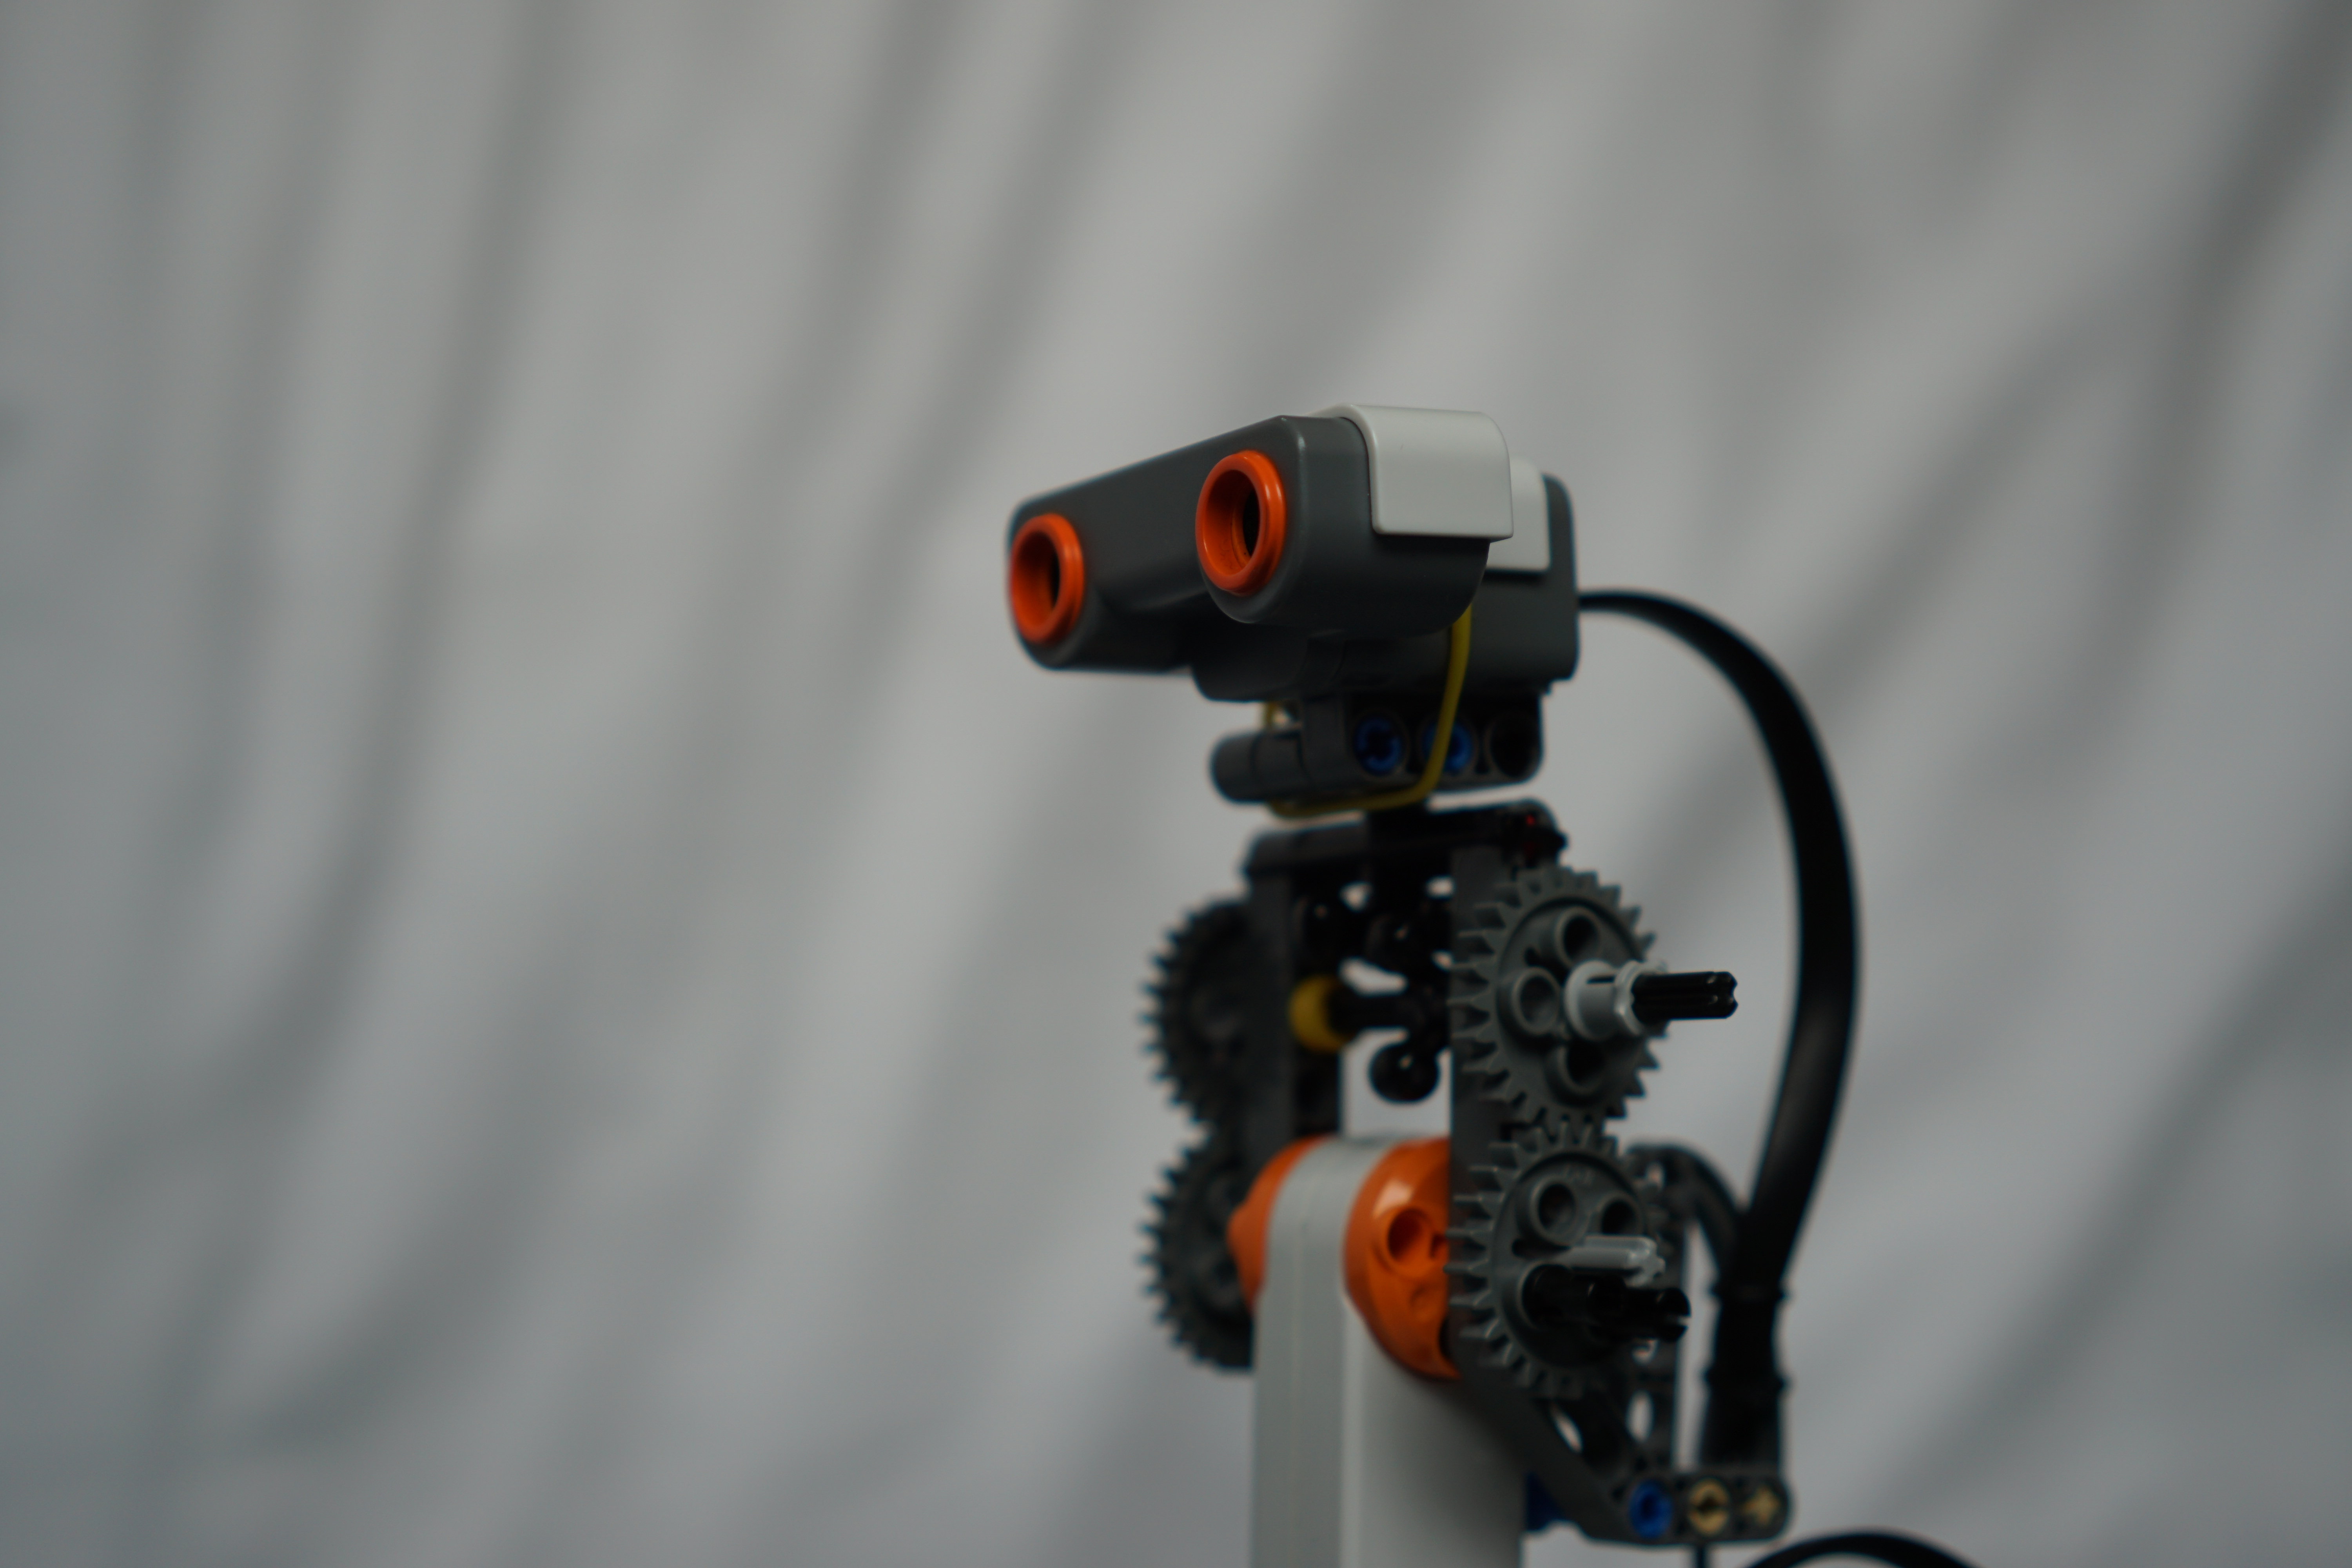
\includegraphics[width=0.5\textwidth]{headshot}
 \caption{Rover Head Sensor}
 \label{fig:stanley-head}
\end{figure}

During development a reactive approach was taken, using the subsumption architecture \citep{wooldridge2009introduction} with emphasis on sensing using multiple layers of perception to allow for informed movement decisions. The use of the subsumption architecture was based on Brooks' thesis that Intelligence is an emergent property of certain complex systems. \citep{brooks1991intelligence} During development this subsumption approach was added into the perception mechanism, during which the rover had to to decide on it's current situation.

\section{Approach}

% The approach describes in detail exactly what you have done. This section is longer, and should ideally include some experiments you set up, for example to determine in what conditions you could get better results from the robot. The approach should be in sufficient detail that another person could replicate your experiments. You may cite other papers here too if you are taking an approach from another paper, or modifying it only slightly.

% Please do mention who shared your robot in the approach section, and the extent to which you worked together. The objective here is to learn. How much you work together is totally up to you so long as you each write your report independently.

% Submissions should be in PDF or HTML, preferably derived from this latex format, certainly in 12 point font. I recommend making HTML by using latex plus htlatex, but you can construct your report using any tool you please. Note that this specification is exactly 2 pages long, so an HTML report should be no longer than this. Figures (both drawn plans and photos) are encouraged for marks and clarity and do not count either for or against page length. The 1–2 pages are counting text only (not citations). But remember, don’t spend too much time on this coursework! You should spend about 19 hours total on each coursework, about 4 of which will be writing up. The coursework should be uploaded to Moodle by 11pm on Friday 3 March at the latest, but feel free to submit it (much) sooner.

% To quantify the outcomes of this coursework, you may want to think about questions such as contrasting the addition of extra control algorithms, changing the physical shape of the robot, or trying different target sonar readings for maintaining a particular distance from the wall in a variety of contexts. These can be quantified in terms of the circuit time for the robot, the success rate, or any other metric you can think of.

% For coursework one, it is quite likely that you will not have initially thought of a hypothesis to test, but will rather just have tried to make the robot work. However, in your exploration (both with the robot and with your reading) you should always be looking to something that seems to make a difference in performance, and then try to capture what that something is. Can you describe it ex you get given how much change you make to some parameter on the robot? Don’t forget to consider things such as the battery charge, operating in daylight, or proximity to other sonar-using robots as possible explanations for strange behaviour.

The initial design of the rover was a simple reflex agent as described by \cite{russell1995modern}. This took the sensor readings, and using transduction converted them to a proximity reading in every direction. This allowed to rover to react to a crash but when recovering from a crash the rover had no context. As a result I settled on \cite{russell1995modern}'s model-based reflex agent. This allows the sensors to modify the state at individual rates, in the final design there were two sensing thread loops, operating at different tick rates, as shown in figure \ref{fig:perception}. One for the sonar which provided slow but accurate readings and one for the other sensors which provided almost instantaneous measurements.

All of the sensor readings were mixed and the closest reading was taken. This was especially important for the front sensor where 3 separate readings were taken from the bump, light and sonar sensor. To improve sensor quality 15 readings were taken every measurement and any reading more than two standard deviations away from the mean were thrown out, and the remainder of the readings were averaged.

\begin{figure}
 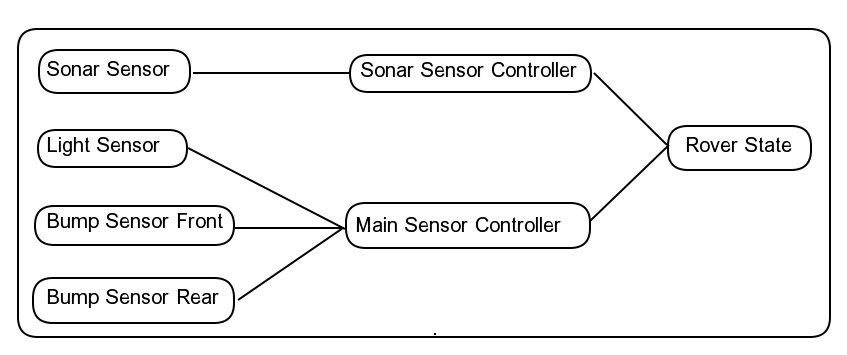
\includegraphics[width=0.5\textwidth]{sensing-diagram}
 \caption{Final Perception Architecture}
 \label{fig:perception}
\end{figure}

In order to control the rover a third thread was started. This read the state and converted the state into a meta-state for the rover. An example of such a state was \emph{TOO\_CLOSE\_TO\_WALL} or \emph{WALL\_NOT\_FOUND}. To determine this state a subsumption architecture used. For example, if the rover was \emph{NEAR} something to the front, it had crashed and it did not matter that \emph{NEAR} an object on the left too. This meta-state was then used in the action planner, which selected the best appropriate action given a meta-state and current states. If the rover was crashed and it was \emph{NEAR} an object to the left. It shouldn't try to reverse to the left.

In addition the meta-state could direct the sonar. If it was following a wall on the left and had found the wall, it could just look left and forward for faster readings. There was no need to update the RHS. This basic system describes the platform for experimentation. The goal was to find if there was an optimal sensing rate.

The rover was run at a tick rate (measurements per second) of 5, 25 and 45. To rate the rover performance during each experiment I measured the number of impacts with the wall as well as marking the number of times it was stuck while navigating the test track shown in fig \ref{fig:area}. The hypothesis is that the rover will perform better with a higher tick rate, but after a certain level, increasing it will no longer have an effect. The former measurement was recorded in software and the later was done by observation. If the rover was stuck in a corner, the experiment was restarted. During each run, the rover was started in the bottom left hand corner of the arena facing the left wall.

\begin{figure}
 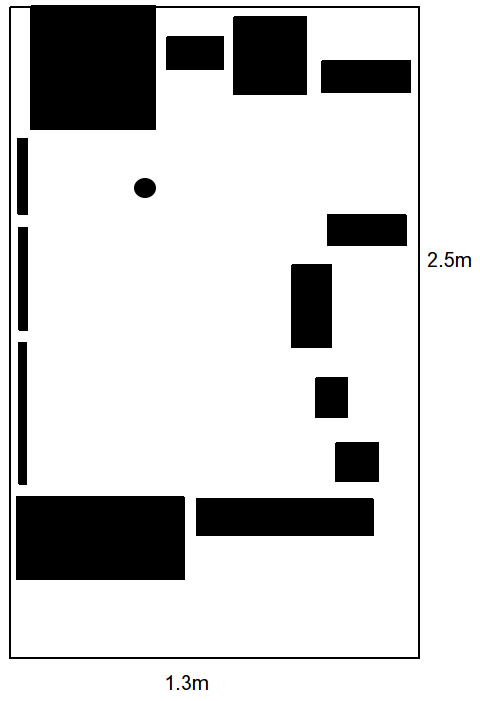
\includegraphics[width=0.5\textwidth]{test-area-layout}
 \caption{Test Area Layout}
 \label{fig:area}
\end{figure}

Throughout the research the rover was shared with Ryan Cullen. In the first part of the coursework the rover resided in my house. I built the rover itself, optimising it's design over several iterations and created the perception system of the code. The software continuously modified proximity readings in the state, indicating how close the rover was to an object in all four cardinal directions. At this point the code was then forked by Ryan and we each developed our own action selection code based on the rover state.

\begin{figure}[b]
 \includegraphics[width=0.5\textwidth]{full}
 \caption{Stanley Rover}
 \label{fig:stanley}
\end{figure}

\section{Results}

% The results section describes the outcomes. This should be purely factual descriptions, including qualitative outcomes, quantitative outcomes and possibly statistics. For example, you could report the average speed around a circuit in two conditions plus standard deviations and a significance test to tell whether you have evidence that the conditions lead to different results. For coursework 1, this must include video. Typically, the results section can be surprisingly short, since the Approach section is the one giving details. Results are purely and only factual outcomes (no alternative facts).

% With respect to your personal results, if you describe a reasonably-well working system in a comprehensible manner you will pass. If you competently fill in all of these sections as described in this specification, you will get at least 55. Getting a mark over 70 requires demonstrating insight, creativity and / or understanding that goes beyond the basics laid out for you in this document. For example, an insightful comment about one or more cited papers supported by evidence from your experience might get you these extra marks. So might a particularly accurate and replicable account of your approach and results.

%

The hypothesis of the experiment was as expected. With this positive result I also ran the experiment after doubling the rover movement speed and found that a higher tick rate actually assisted the rover at higher speeds, leading to the conclusion that the faster the rover moves, the faster it needs to sense the environment around it.

The results for one lap were very noisy, but as the rover was required to do 10 laps, both 10 lap runs were within 5 bumps / lap of each other.

\begin{table}
\centering
\caption{Test Results}
\label{my-label}
\begin{tabular}{|l|c|c|c|}
\hline
Tickrate         & 5  & 25 & 45 \\ \hline
Bumps/lap @ Slow & 23 & 14 & 16 \\ \hline
Bumps/lap @ Fast & 53 & 46 & 26 \\ \hline
\end{tabular}
\end{table}

The video found at \url{https://youtu.be/LOPdO0w1Uec} depicts the start of a trail run.

\section{Discussion}

% The discussion is the most discursive part of your paper, it may include speculation. You should discuss the extent to which your results addressed the questions described in your introduction, and what the results imply about your own work and AI or robotics more broadly. You might suggest other experimental protocols that could have given different results and lessons learned. This can be a longer section, and may again include citations if you compare or contrast to other published accounts.

The results I got closely matched the hypothesis, however, I was not able to increase the sensing speed of the sonar due to physical limitations, which is the key part of the navigation logic. I suspect that adding a second sonar that did not require physical movement for sensing would greatly increase the navigation capabilities of the rover.

During the experiments I tried to run the rover in as fixed of an environment as possible, as I found the light sensor was very susceptible to sunlight and found that closing the blinds made runs at different times of day much more consistent.

In general I think that to improve navigation, sensing and decision loops should always be run as fast as possible, and the faster the movement the more important this is. This extremely important in applications such as quadcopters where loop times affect flight characteristics \citep{betaflight}

\section{Conclusion}

% The conclusion is just one paragraph. After possible digressions in the discussion, you should come back to restate exactly what you tried to do (brief summary of the introduction), what the outcome was (brief summary of the results), and what you can certainly state as a result of this (the implications of the results in light of the introduction.)

This research set out to find the impact of sensing speed on the navigation of rovers. The results show that a faster sensing loop results in more accurate navigation, although, after a certain accuracy is reached returns diminish.

When deciding on sensing loop speeds, this level should be reached and not surpassed, as going too high might take compute cycles away from the planning loop.

\bibliography{lejos-writeup}

\end{document}
